\documentclass{article}
\usepackage[utf8]{inputenc}
\usepackage[T1]{fontenc}
\usepackage[spanish,es-nodecimaldot]{babel}
\usepackage{amsmath,amsfonts,amssymb,amstext,amsthm,amscd}
\usepackage{latexsym}
\usepackage{graphicx}
\graphicspath{{figures/}{./}}
\usepackage{subfig}
\usepackage{float}
\usepackage{dcolumn}
\usepackage{bm}
\newcounter{itemR}

\usepackage{fancyhdr}
\usepackage{multicol}
\usepackage{caption}
\usepackage{url}
\captionsetup[figure]{belowskip=0pt}

% ------------------------------------------------------------------------------------------------------------------------------------------------------


\setlength{\headheight}{15.2pt}
\usepackage[paperwidth=8.5in, paperheight=11.0in, top=1.0in, bottom=1.0in, left=1.0in, right=1.0in]{geometry}

\captionsetup[figure]{belowskip=0pt}
\setlength{\intextsep}{4pt plus 2pt minus 2pt}
\setlength{\textfloatsep}{4pt plus 2pt minus 2pt}
\setlength{\floatsep}{4pt plus 2pt minus 2pt}
\setlength{\abovecaptionskip}{4pt}
\pagestyle{fancyplain}
\fancyhead[LE,RO]{Espejo de Fresnel}
\fancyhead[CE,CO]{}
\fancyhead[RE,LO]{O26-LFA3032-1}
\fancyfoot[LE,RO]{\thepage}
\fancyfoot[CE,CO]{\'Optica Experimental, UDLAP}
\fancyfoot[RE,LO]{}

% ------------------------------------------------------------------------------------------------------------------------------------------------------

\begin{document}

\fancypagestyle{plain}{
    \renewcommand{\headrulewidth}{1pt}
    \renewcommand{\footrulewidth}{1pt}
}

\renewcommand{\footrulewidth}{1pt}
\renewcommand{\tablename}{Tabla}

% ------------------------------------------------------------------------------------------------------------------------------------------------------

\title{Experimento del espejo de Fresnel\\ \small{}}
\author{\small Alan Ivan Ortega Contreras \footnote{184544; alan.ortegacs@udlap.mx}, Luz Stefanía Pérez Huesca \footnote{183848; luz.perezha@udlap.mx}, Ángel Gabriel Munguía Velázquez \footnote{185518; angel.munguiavz@udlap.mx}\\
    \small Depto.~de Actuaría, Física y Matemáticas, Universidad de las Américas Puebla, Puebla, M\'exico 72810}
\date{\small{\today}}

\maketitle

% ------------------------------------------------------------------------------------------------------------------------------------------------------

\begin{abstract}
Se estudió la interferencia de dos fuentes virtuales coherentes mediante el espejo de Fresnel. Se midió la separación media entre máximos consecutivos y se utilizó una lente de formación de imágenes para determinar la separación geométrica entre las dos fuentes virtuales generadas. A partir de estas mediciones se obtuvo una longitud de onda de $(670\pm70)\ \mathrm{nm}$, con un error porcentual de $6.3\%$ respecto al valor nominal de $632.8\ \mathrm{nm}$. El patrón observado corroboró el fenómeno de interferencia geométrica entre dos trayectorias reflejadas.

\medskip
\noindent\textit{Keywords:} interferencia, espejo de Fresnel, fuentes virtuales, longitud de onda, láser He-Ne.
\end{abstract}

% ------------------------------------------------------------------------------------------------------------------------------------------------------

\begin{multicols*}{2}
\raggedcolumns

\section*{Objetivo y metas específicas}\label{Objetivo}                               
El propósito general de la práctica consistió en observar la interferencia entre dos fuentes de luz virtuales mediante el espejo de Fresnel. El objetivo principal fue determinar la longitud de onda del láser mediante el promedio de la separación entre máximos consecutivos de intensidad $d$ y la distancia de separación proyectada de los puntos $A$. 

\section*{Introducción}
La naturaleza de la luz fue un tema de gran controversia durante mucho tiempo en la física; en 1690, Christiaan Huygens interpretó la luz como un fenómeno ondulatorio, mientras que en 1704, Isaac Newton describió el haz de luz como una corriente de partículas. Esta contradicción histórica fue resuelta posteriormente por la mecánica cuántica con el surgimiento de la idea de la dualidad onda-partícula. 

Uno de los arreglos clásicos para estudiar el comportamiento ondulatorio es el espejo de Fresnel, el cual tiene como objetivo principal generar dos fuentes de luz virtuales y coherentes a través de la reflexión de una fuente de luz puntual. La superposición de estas trayectorias permite observar directamente el fenómeno de interferencia sorteando el problema de la incoherencia que presentan dos fuentes luminosas independientes.

\section*{Marco teórico}
En el montaje experimental del espejo de Fresnel, el haz reflejado por dos espejos planos ligeramente inclinados genera dos ondas coherentes que se originan en las fuentes virtuales $S_1'$ y $S_2'$. El enésimo máximo de intensidad ocurre cuando la diferencia de trayectoria óptica ($\Delta s$) de las dos ondas cumple con la condición $\Delta s = n \cdot \lambda$.

\begin{center}
\begin{minipage}{\linewidth}
    \centering
    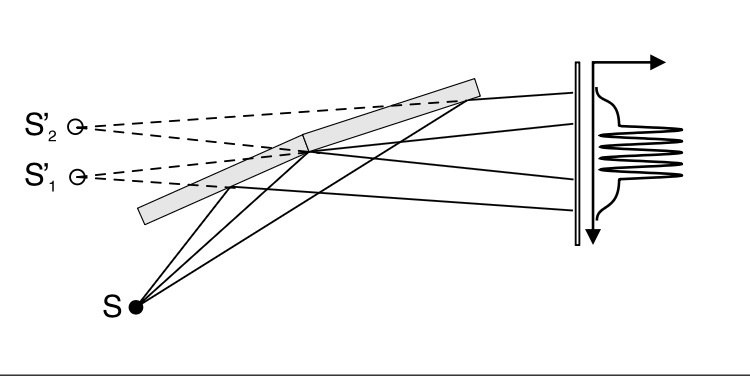
\includegraphics[width=\linewidth,height=5cm,keepaspectratio]{Diagrama_Fresnel.png}
    \captionof{figure}{Diagrama de rayos del espejo de Fresnel.}
    \label{Fig:montaje_teorico}
\end{minipage}
\end{center}

Para una distancia grande $L$ entre las fuentes virtuales y la pantalla de observación, se puede calcular la longitud de onda ($\lambda$) de la luz utilizada (láser He-Ne) a partir de la distancia $a$ entre las fuentes virtuales y la distancia $d$ medida entre las líneas de interferencia contiguas:

\begin{equation}
    \lambda = a \cdot \frac{d}{L}
    \label{ec:longitud_onda_fresnel}
\end{equation}

Para utilizar esta ecuación, la distancia $a$ entre las fuentes de luz virtuales debe determinarse generando imágenes proyectadas de dichas fuentes sobre una pantalla. A partir de la geometría de los triángulos semejantes formados en la proyección del experimento, midiendo la distancia $A$ entre las imágenes proyectadas por una segunda lente, se obtiene la siguiente relación:

\begin{equation}
    a = A \cdot \frac{L_1}{L_2}
    \label{ec:distancia_fuentes_virtuales}
\end{equation}
donde $L_1$ es la distancia desde las fuentes virtuales a la lente de proyección y $L_2$ es la distancia desde dicha lente a la pantalla. Al combinar ambas ecuaciones se obtiene un método puramente geométrico para estimar la longitud de onda.

\begin{center}
\begin{minipage}{\linewidth}
    \centering
    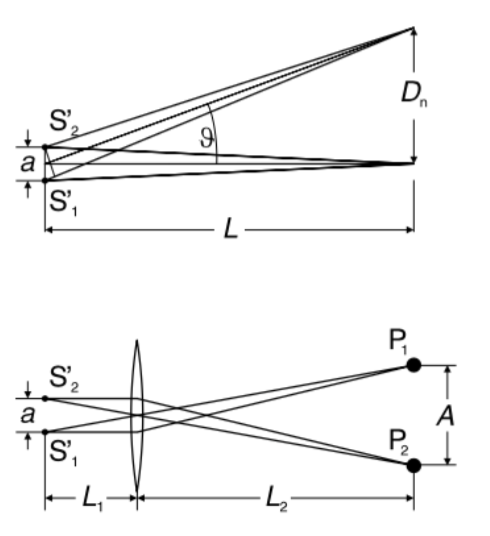
\includegraphics[width=\linewidth,height=5cm,keepaspectratio]{trayectoria.png}
    \captionof{figure}{Trayectoria del haz para la interferencia (superior) y proyección de las fuentes virtuales con la lente (inferior).}
    \label{Fig:diagrama_proyeccion}
\end{minipage}
\end{center}


\section*{Materiales y equipos}\label{Material}                            
\begin{itemize} 
    \item Kit de espejo de Fresnel
        \subitem 1 láser He-Ne, linealmente polarizado (632.8 nm)
        \subitem 1 lente $f=+5\ \mathrm{mm}$
         \subitem 1 lente $f=+200\ \mathrm{mm}$
        \subitem 1 pantalla traslúcida
        \subitem 1 espejo de Fresnel ajustable
        \subitem 1 banco óptico
\end{itemize}

\section*{Metodología}\label{Metodologia}                

Se montó el arreglo experimental; en primer lugar, se ajustó el láser He-Ne al extremo del banco óptico. Acto seguido se colocó la lente de $f=+5\ \mathrm{mm}$ frente al láser para ensanchar el haz. Después se colocó el espejo de Fresnel alineado paralelamente al eje óptico de modo que el haz ensanchado incidiera en la arista de separación de los semi-espejos. Se posicionó la segunda lente de $f=+200\ \mathrm{mm}$ cerca del espejo. 

Se movió la perilla del espejo para ajustar el ángulo de inclinación hasta visualizar dos puntos de intensidad aproximadamente igual en la pantalla translúcida. Mediante los ajustes se fijó la distancia de separación entre las imágenes proyectadas ($A$) a aproximadamente 5 mm y se midió finamente con un vernier. 

Se registró la distancia desde el centro de la lente de proyección a la pantalla ($L_2$) y la distancia entre la lente de ensanchamiento y la lente de proyección ($L_0$). Dado que la fuente puntual real coincide con el foco de la lente de $5\ \mathrm{mm}$, la distancia $L_1$ se calculó geométricamente restando este foco a $L_0$.

\begin{center}
\begin{minipage}{\linewidth}
    \centering
    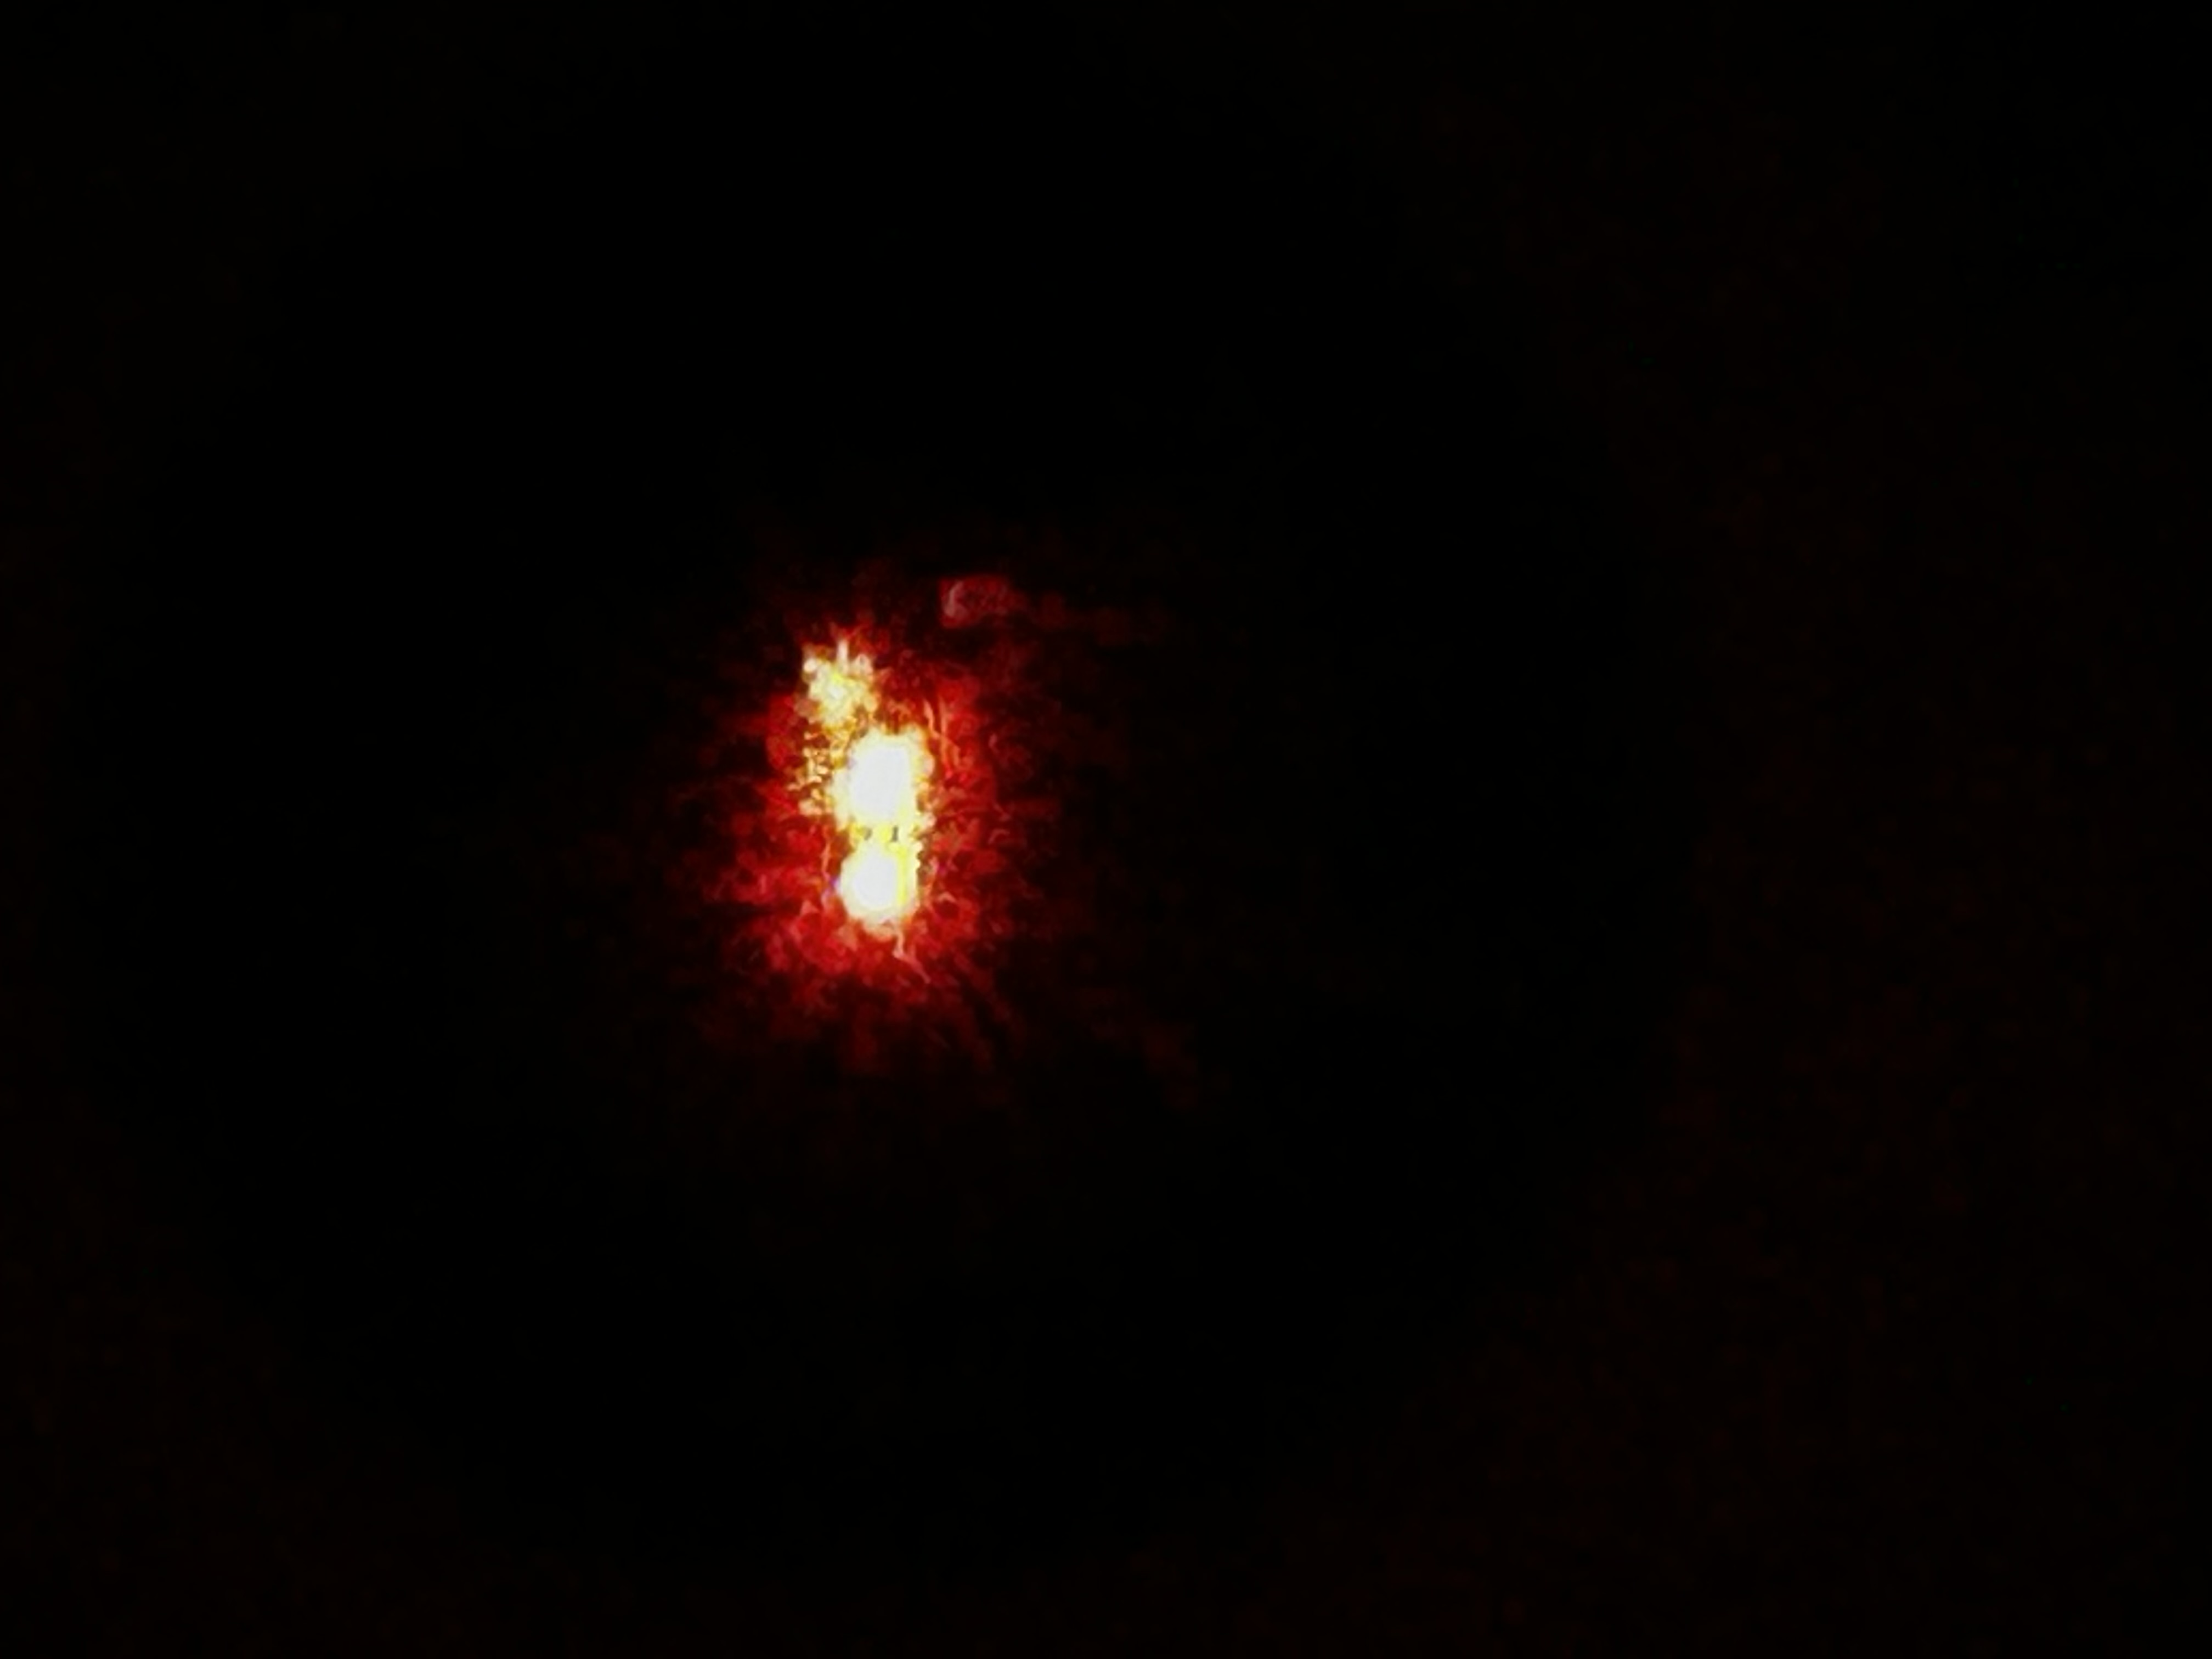
\includegraphics[width=\linewidth,height=5cm,keepaspectratio]{IMG_5736.jpeg}
    \captionof{figure}{Fuentes virtuales proyectadas en la pantalla traslúcida.}
    \label{Fig:puntos_pantalla}
\end{minipage}
\end{center}

Se retiró la lente de $200\ \mathrm{mm}$ para permitir que los haces divergentes interfirieran directamente sobre la pantalla de observación.

\begin{center}
\begin{minipage}{\linewidth}
    \centering
    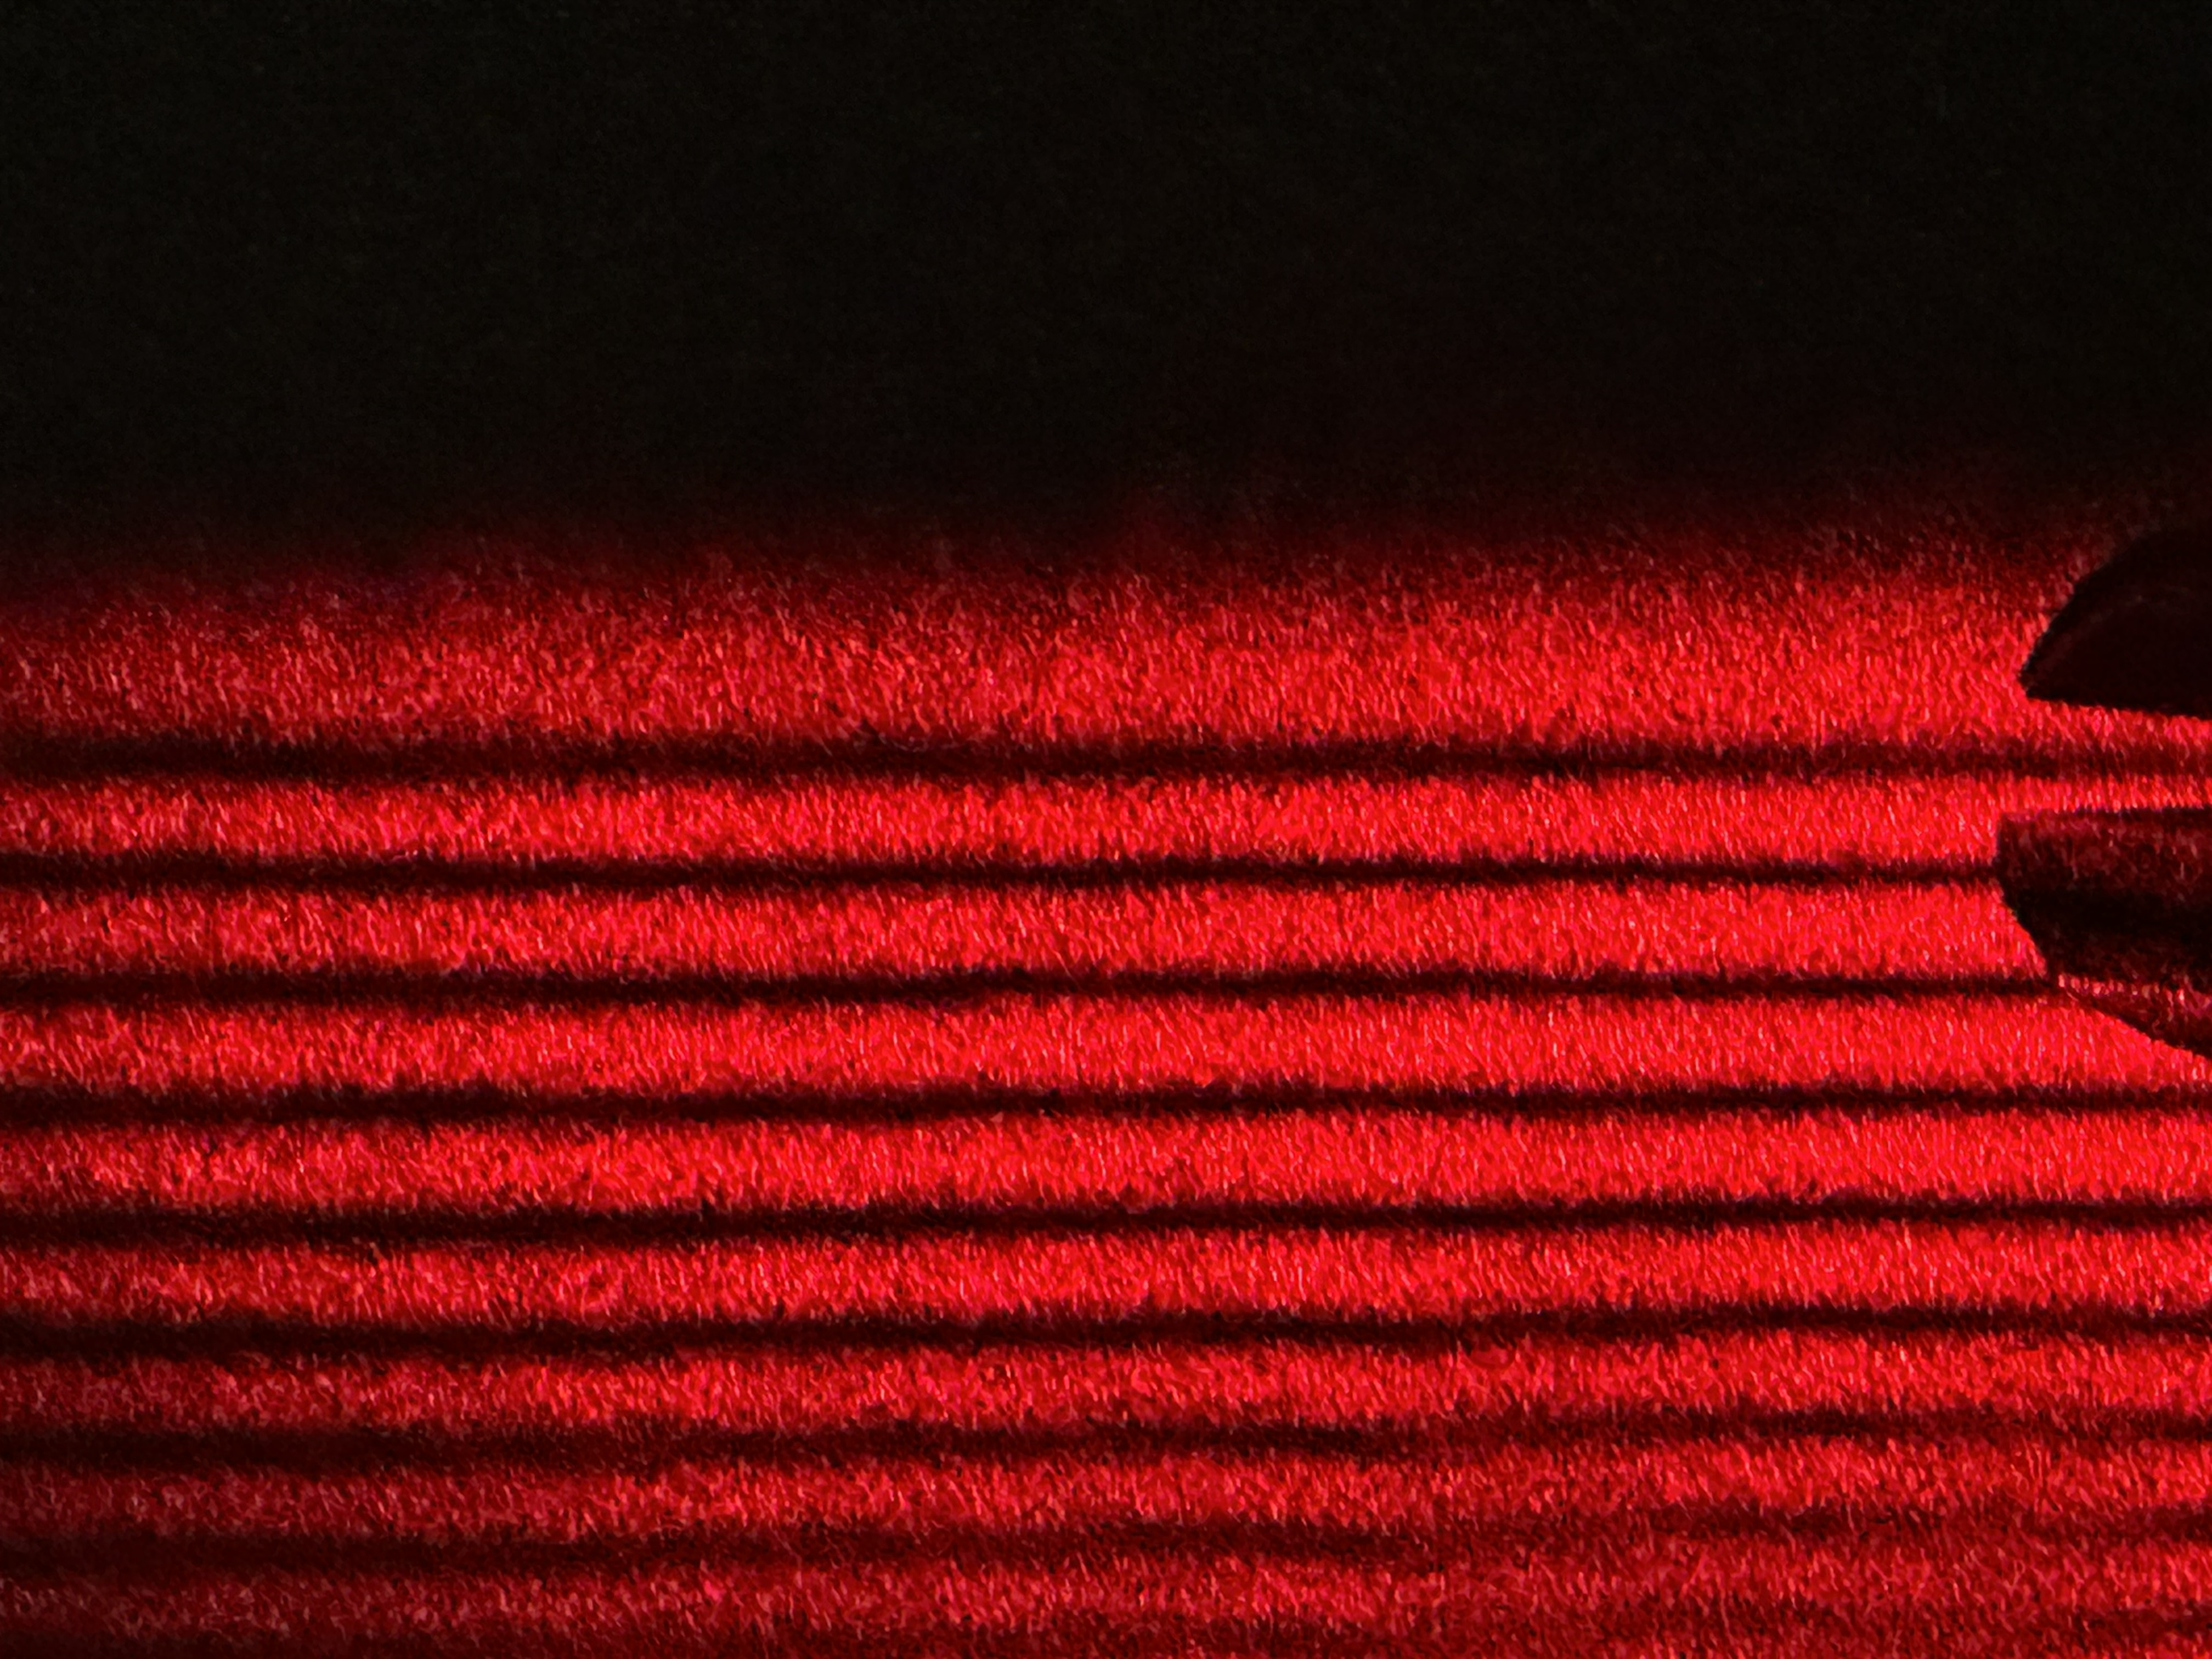
\includegraphics[width=\linewidth,height=5cm,keepaspectratio]{IMG_5734.jpeg}
    \captionof{figure}{Patrón de interferencia observado.}
    \label{Fig:patron}
\end{minipage}
\end{center}

Finalmente, se midieron cinco separaciones $d_k$ entre máximos consecutivos de intensidad utilizando un vernier, se obtuvo su promedio, y se propagaron las incertidumbres para calcular la longitud de onda experimental y compararla con el valor de referencia.

\begin{center}
\begin{minipage}{\linewidth}
    \centering
    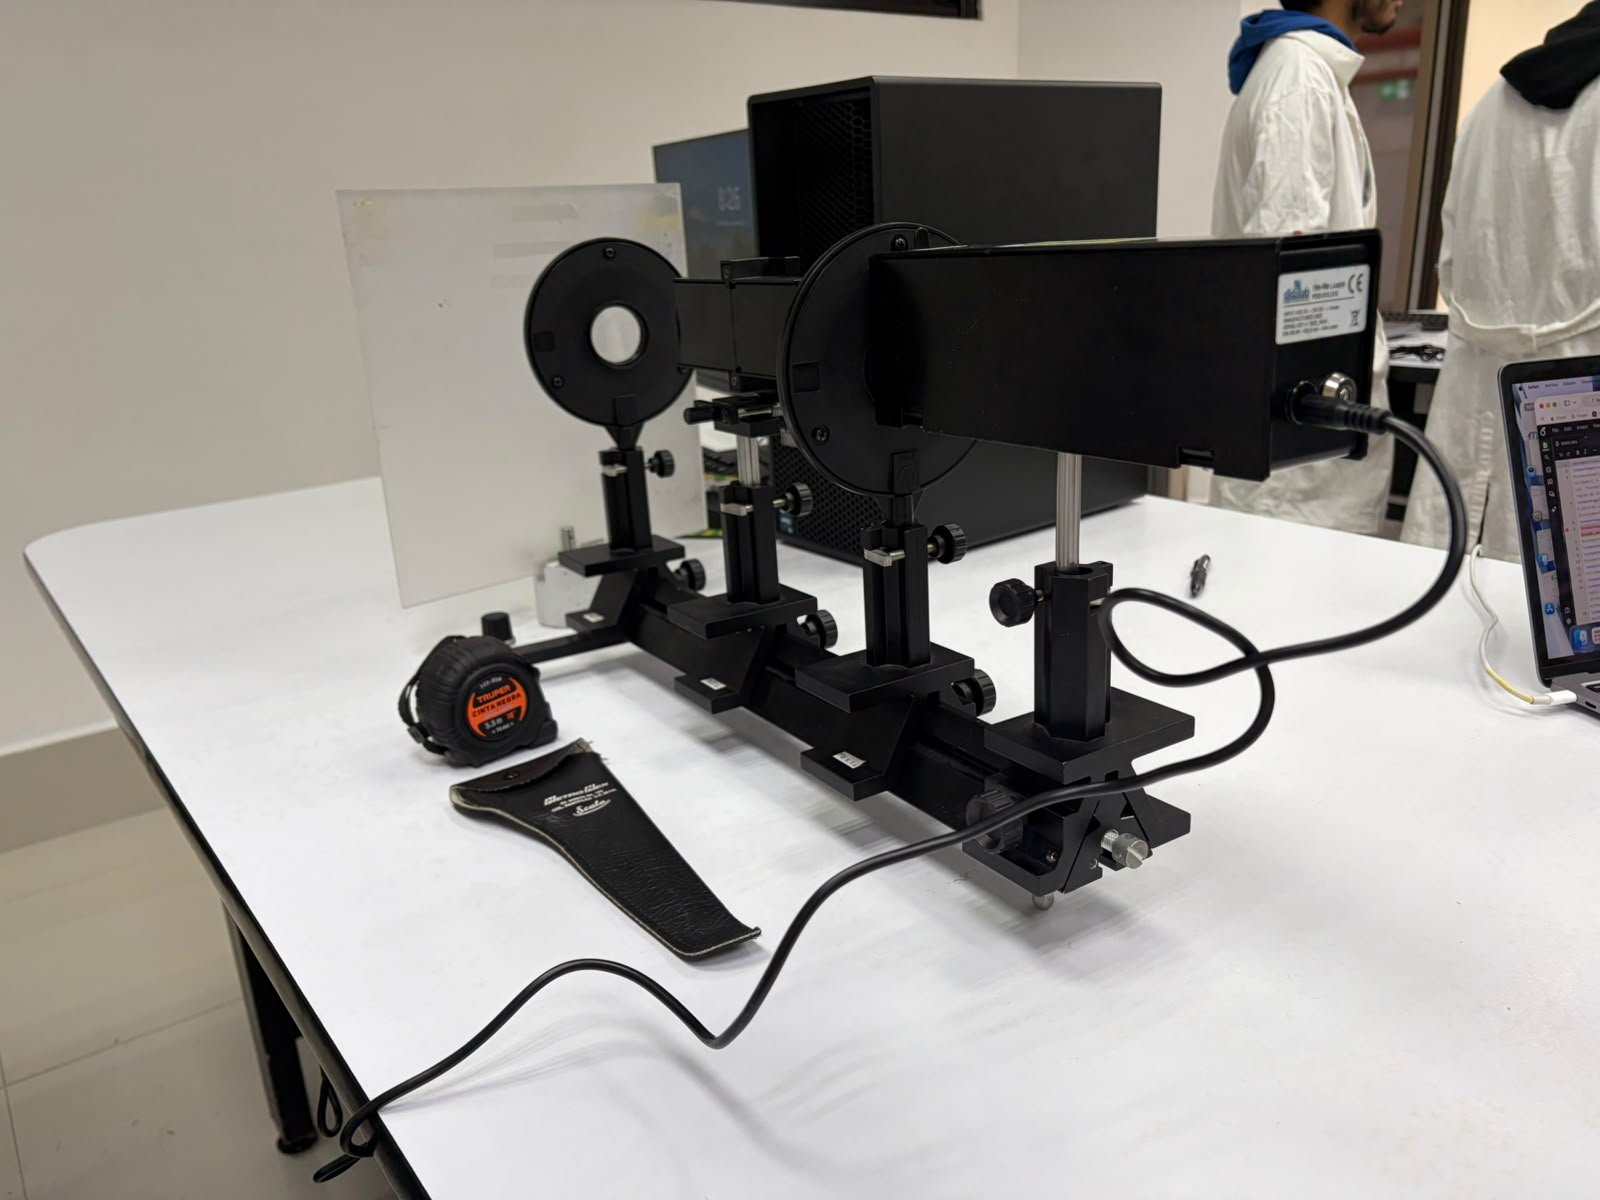
\includegraphics[width=\linewidth,height=5cm,keepaspectratio]{PHOTO-2026-10-02-07-00-35.jpg}
    \captionof{figure}{Montaje final del arreglo experimental.}
    \label{Fig:montaje_real}
\end{minipage}
\end{center}

\section*{Resultados y análisis}\label{Resultados}

La Tabla~\ref{tab:franjas} presenta las cinco mediciones tomadas para las separaciones contiguas entre franjas.

\begin{center}
\begin{minipage}{\linewidth}
\centering
\begin{tabular}{|c|c|}
\hline
Medición $k$ & $d_k\pm0.01\ (\mathrm{mm})$\\
\hline
1 & 0.36\\
2 & 0.46\\
3 & 0.50\\
4 & 0.32\\
5 & 0.32\\
\hline
\end{tabular}
\captionof{table}{Separaciones entre máximos consecutivos de intensidad.}
\label{tab:franjas}
\end{minipage}
\end{center}

\begin{center}
\begin{minipage}{\linewidth}
\centering
\begin{tabular}{|c|c|}
\hline
Distancia  & Valor (cm)\\
\hline
$A$ & $0.50\pm 0.01$ \\
$L_0$& $29.00\pm 0.05$ \\
$L_2$ & $78.00\pm 0.05$ \\
\hline
\end{tabular}
\captionof{table}{Distancias geométricas registradas en el montaje.}
\label{tab:distancias}
\end{minipage}
\end{center}

Para $N=5$, el promedio en milímetros y su incertidumbre estadística de la media se calcularon como:
\begin{align}
\bar d &=\frac{1}{N}\sum_{k=1}^{N}d_k,\\
\sigma_d&=\sqrt{\frac{1}{N-1}\sum_{k=1}^{N}(d_k-\bar d)^2},\\
\sigma_{\bar d}&=\frac{\sigma_d}{\sqrt N}.
\end{align}
Considerando una cifra significativa para la incertidumbre, el espaciamiento medio resultó en:
\begin{equation}
\bar d=(0.39\pm0.04)\ \mathrm{mm}.
\end{equation}

Las otras magnitudes empleadas (convertidas a milímetros) son $A = (5.0 \pm 0.1)\ \mathrm{mm}$, $L_0 = (290.0 \pm 0.5)\ \mathrm{mm}$ y $L_2 = (780.0 \pm 0.5)\ \mathrm{mm}$. 
Sabiendo que la fuente puntual está en el foco de la lente expansora, tenemos $L_1 = L_0 - 5\ \mathrm{mm} = 285.0\ \mathrm{mm}$. Por consiguiente, la distancia total de la fuente a la pantalla es $L = L_1 + L_2 = 1065.0\ \mathrm{mm}$.

Calculamos primero la separación intrínseca de las fuentes virtuales $a$:
\begin{equation}
a = A \cdot \frac{L_1}{L_2} = 5.0\ \mathrm{mm} \cdot \frac{285.0\ \mathrm{mm}}{780.0\ \mathrm{mm}} \approx 1.83\ \mathrm{mm}.
\end{equation}

Sustituyendo los valores en la ecuación de interferencia geométrica, la longitud de onda obtenida es:
\begin{equation}
\lambda = a \cdot \frac{\bar d}{L} = 1.827\ \mathrm{mm} \cdot \frac{0.392\ \mathrm{mm}}{1065.0\ \mathrm{mm}} = 672.4\ \mathrm{nm}.
\end{equation}

La incertidumbre de la longitud de onda se propagó asumiendo variables independientes mediante derivadas parciales:
\begin{equation}
\delta\lambda=\lambda\sqrt{\left(\frac{\delta A}{A}\right)^2+\left(\frac{\delta\bar d}{\bar d}\right)^2+\dots}
\end{equation}
Al evaluar la propagación, las contribuciones dominantes provienen de las mediciones de $A$ y $\bar d$. Resolviendo se obtiene $\delta\lambda \approx 70\ \mathrm{nm}$. Redondeando la incertidumbre a una cifra significativa, el resultado experimental se reporta como:
\begin{equation}
\boxed{\lambda=(670\pm70)\ \mathrm{nm}.}
\end{equation}

Se adoptó como referencia $\lambda_{\mathrm{ref}}=632.8\ \mathrm{nm}$, correspondiente al láser He-Ne. El error porcentual se calculó con el resultado previo al redondeo:
\begin{equation}
\begin{split}
\%\mathrm{error}
&=\frac{|\lambda_{\mathrm{exp}}-\lambda_{\mathrm{ref}}|}{\lambda_{\mathrm{ref}}}\times100\%\\
&=\frac{|672.4-632.8|}{632.8}\times100\%\\
&=6.3\%.
\end{split}
\end{equation}

\subsection*{Análisis del resultado}
El valor experimental de longitud de onda obtenido ($670\ \mathrm{nm}$) guarda una excelente correlación con la longitud de onda real del láser He-Ne ($632.8\ \mathrm{nm}$). Con un error del $6.3\%$, la medición se ubica dentro de los márgenes de la incertidumbre propagada ($\pm 70$ nm). La ligera sobreestimación se debe principalmente a la dificultad mecánica y visual de medir franjas submilimétricas ($\sim 0.39$ mm) a simple vista sobre una pantalla de proyección empleando un vernier. Dicha limitación podría haberse reducido al acatar la recomendación de usar un $L_2 > 2$ m para amplificar y espaciar el patrón.

\section*{Conclusiones}
En esta práctica se evaluó el comportamiento ondulatorio de la luz a través de la interferencia generada por el espejo de Fresnel. El marco geométrico de los triángulos semejantes permitió proyectar las fuentes virtuales en la pantalla y medir una separación efectiva ($a \approx 1.83\ \mathrm{mm}$). El cálculo experimental de la longitud de onda dio como resultado $(670\pm70)\ \mathrm{nm}$, con un error del $6.3\%$ en contraste con los $632.8\ \mathrm{nm}$ nominales. Estos resultados validan cuantitativamente la relación entre el espaciamiento de las franjas y la longitud de onda, demostrando la eficacia del arreglo para producir fuentes virtuales espacialmente coherentes.

\begingroup
\interlinepenalty=10000
\begin{thebibliography}{9}
\bibitem{LD_Physics}
LD DIDACTIC GmbH,
\emph{Interference at a Fresnel's mirror with an He-Ne laser},
Physics Leaflets P5.3.2.1, pp.~1--3.

\bibitem{Laser}
LEYBOLD DIDACTIC GmbH,
\emph{He-Ne laser, linearly polarised (471 830)},
Instruction sheet, 06/04-W97-Kem, pp.~1--2.
\end{thebibliography}
\endgroup
\end{multicols*}
\end{document}